\documentclass[letterpaper,11pt]{article}
\usepackage[utf8x]{inputenc}
\usepackage{enumerate}
\usepackage{enumitem}
\usepackage{fullpage}
\usepackage{amsmath}

\usepackage{pgf}
\usepackage{tikz}
\usepackage{circuitikz}
\usepackage{siunitx}

%opening
\title{Final Exam \\ Classical Mechanics \\ Physics 601 (Fall 2013)}
\date{Thursday December 12, 2013, 9am}

\begin{document}

\maketitle

\paragraph*{Instructions}
\begin{itemize}
 \item This exam is governed by \textbf{William \& Mary Honor Code}.
 \item This exam is to be completed \textbf{individually}.
 \item This exam is `open notes:' you are allowed to use the textbook, your homework assignments, your personal notes, and one page of additional printed material.
 \item Carefully explain each step in your answer.
 \item Calculators are not needed for this exam.
 \item Write your \textbf{name on every page}.
 \item Write your responses on \textbf{single-sided} letter paper.
\end{itemize}

\pagebreak

\paragraph*{Lagrangian Mechanics}
\begin{enumerate}
 \item A point mass $m_1$ slides frictionlessly along a curve $y = f(x)$.  Assume $f(-x) = f(x)$ is an even function with a single minimum at $x = 0$, and that $f''(x) > 0$.  Affixed to the mass is a rigid rod of length $\ell$ with at the other end a second point mass $m_2$.  The entire system moves under the influence of gravity.  Choose as a set of generalized coordinates the set ${x,y,\theta}$, where $(x,y)$ are the Cartesian coordinates of the mass $m_1$, and $\theta$ is the angle between the rod and the downward vertical. [40 points]
 \begin{enumerate}
  \item Treat the condition $y = f(x)$ as a constraint.  Find four equations for the four unknowns $x$, $y$, $\theta$, and $\lambda$, where $\lambda$ is the Lagrange multiplier.  Without solving these equations, describe how you would determine the force of constraint normal to the wire. [10 points]
  \item Treat the system without the constraint formalism, using the generalized coordinates $x$ and $\theta$ only.  Find the Lagrangian $L(x,\theta,\dot{x},\dot{\theta},t)$.  Find the equilibrium values $(x^*,\theta^*)$ and determine the mass and potential matrices $M$ and $V$ (remember that $f(x)$ is an even function). [10 points]
  \item Consider the specific case $f(x) = x^2/2b$.  Define $\Omega_0 = \sqrt{g/b}$ and $\Omega_1 = \sqrt{g/\ell}$.  Find a general expression for the normal mode frequencies $\omega_\pm$.  Find the eigenvectors $z^\pm$ (you do not need to normalize them). [15 points]
  \item Find and interpret the limits of the frequencies $\omega_\pm$ for small $m_1$, and small $m_2$. [5 points]
  \begin{center}
   \begin{tikzpicture}[domain=-2.5:2.5]
    \draw[->] (-4.2,0) -- (4.2,0) node[right] {$x$};
    \draw[->] (0,-1.2) -- (0,2.8) node[left] {$y$};
    \draw plot[id=x] function{x*x*x*x/21} node[right] {$f(x)$};
    \filldraw (2,0.762) circle(3pt) node[right] {$m_1$};
    \begin{scope}[shift={(2,0.762)}]
     \draw (0,0) -- (-90:2);
     \draw (0,0) -- (-60:2);
     \draw[->] (0,0) -- (-90:1.2) arc (-90:-60:1.2) node[below left] {$\theta$};
     \filldraw (-60:2) circle (3pt) node[right] {$m_2$};
    \end{scope}
   \end{tikzpicture}
  \end{center}
 \end{enumerate}
\end{enumerate}

\paragraph*{Hamiltonian Mechanics}
\begin{enumerate}[resume]
 \item In the case of a time-dependent Hamiltonian $H\left(p,q;\lambda(t)\right)$ where the time-dependence is due to a parameter $\lambda$ that slowly varies in time, the action $J$ belongs to a class of observables known as \emph{adiabatic invariants}.  The change in $\lambda$ is said to be \emph{adiabatic} if the change $\Delta\lambda$ is slow compared to the period of the motion, or
 \begin{equation*}
  |\Delta\lambda| = |\dot\lambda| \Delta t = |\dot\lambda| \frac{2\pi}{\omega} \ll |\lambda|.
 \end{equation*}
 It can be shown that the action $J$ is \emph{conserved} for changes in the parameter $\lambda$ that satisfy this \emph{adiabatic condition}.

 At the first international Solvay congress in 1911, the following question was posed: how would the energy of a simple pendulum change if the length $\ell$ is changed slowly.  Model the simple pendulum with small amplitude as a harmonic oscillator $H\left(p,q;\omega(t)\right)$, and determine how the following quantities change when the length is \emph{doubled} adiabatically: [10 points]
 \begin{itemize}
  \item the total energy $E$ of the harmonic oscillator,
  \item the amplitude $\theta_{max}$ of the pendulum.
 \end{itemize}
\end{enumerate}

\paragraph*{Small Oscillations}
\begin{enumerate}[resume]
 \item Consider the following coupled $LC$ circuit where $I_{1,2} = dQ_{1,2}/dt$ is the current flowing in a loop of the circuit, $L$ is the inductance of the inductor, and $C$ is the capacitance of the capacitor.  By analogy to mechanical oscillators, the inductance plays the role of an inertial mass, the capacitance plays the role of a spring constant.  The kinetic energy in an inductor is $\frac{1}{2} L I^2$, the potential energy in a capacitor is $\frac{1}{2 C} Q^2$.  The voltage across an inductor is $L \frac{d I}{d t}$, the voltage across a capacitor is $Q/C$.
 \begin{center}
  \begin{circuitikz}
   \draw (0,3) to (4,3);
   \draw (0,0) to[L, i=$I_1$, l=$L$] (0,3);
   \draw (0,0) to[C, l=$C$] (2,0);
   \draw (2,0) to[C, l=$C$] (4,0);
   \draw (4,0) to[L, i=$I_2$, l=$L$] (4,3);
   \draw (2,0) to (2,1);
   \draw (2,3) to[C, l=$C$] (2,1);
  \end{circuitikz}
 \end{center}
 \begin{enumerate}
  \item Determine the Lagrangian for this circuit, and show that the correct Kirchhoff equations can indeed be derived. [10 points]
  \item Treating the Lagrangian\footnotemark{} as a small oscillations problem, what are the frequencies of oscillation and the normal modes for this circuit when the currents and charges are small? [10 points]
  \footnotetext{For partial credit, use this \emph{incorrect} Lagrangian $L(I_1,I_2,Q_1,Q_2) = \frac{1}{2} L (I_1^2 + I_2^2) - \frac{1}{2 C} \left(Q_1 + Q_2\right)^2$}
 \end{enumerate}
\end{enumerate}

\paragraph*{Rigid Bodies}
\begin{enumerate}[resume]
 \item Consider a ``rolling top'' that consists of two identical solid metal spheres of radius $R$ that are point-welded together.
 \begin{center}
  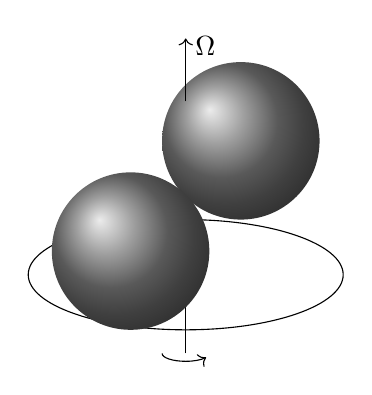
\begin{tikzpicture}
   \draw (-0.3,-2)[->] arc (180:330:0.3 and 0.1);
   \draw (0,-1) ellipse (2 and 0.7);
   \shade[ball color=gray] ( 0.7, 0.7) circle (1);
   \draw (0,-2) -- (0,0);
   \draw (0,1.2)[->] -- (0,2) node[very near end,right] {$\Omega$};
   \shade[ball color=gray] (-0.7,-0.7) circle (1);
  \end{tikzpicture}
 \end{center}
 Determine the principal moments of inertia of this top with respect to the center of mass. [10 points]
\end{enumerate}

%  \item Mechanical tops should be familiar territory to any physics graduate student.  In practice a symmetric top with a fixed contact point with the floor experiences significant rotational friction which will slow it down.  Since the invention of the wheel we know that rolling without slipping is not subject to this frictional energy loss.
% 
%  Consider the ``rolling top'' that consists of two metal spheres of radius $R$ that are point-welded together.  When we spin up this rolling top, the contact point will not be fixed, nor will it be on the symmetry axis of the top.  In steady motion, ignoring the second-order effects of nutation, the top rolls without slipping on a circular trajectory around the center of mass at the weld-joint. Although this top does not have a physical fixed point, we can think of it as having a ``virtual'' fixed point where $\Omega$ and $\omega_3$ intersect\footnotemark{}.  Using the distance $\ell$ between this virtual fixed point and the center of mass, the treatment of the symmetric top with a fixed point in a gravitational field remains unchanged.
%  \footnotetext{Alternatively, imagine a massless rod that connects the top to the fixed point.}
% 
%  \begin{center}
%   \begin{tikzpicture}
%    \draw (-0.3,-2)[->] arc (180:330:0.3 and 0.1);
%    \draw (0,-1) ellipse (2 and 0.7);
%    \shade[ball color=gray] ( 0.7, 0.7) circle (1);
%    \draw (0,-2) -- (0,0);
%    \draw (0,1.2)[->] -- (0,2) node[very near end,right] {$\Omega$};
%    \shade[ball color=gray] (-0.7,-0.7) circle (1);
%   \end{tikzpicture}
%   \qquad
%   \begin{tikzpicture}
%     \draw[->] (-2.2,0) -- (2.2,0) node[right] {$r$};
%     \draw[->] (1.2,-0.4) -- (1.2,3.6) node[left] {$\Omega$};
%     \draw (0,-0.4) -- (0,2.3);
%     \draw (0.4,-0.4) node[right] {$\rho$};
%     \draw (-0.71,-0.4) -- (-0.71,1);
%     \draw (0.4,2.0) node[right] {$\ell$};
%     \begin{scope}[shift={(0,1.71)}]
%      \draw[->] (0,0) -- (45:2.5) node[right] {$\omega_3$};
%      \draw (0,0.4)[->] arc (90:45:0.4) node[above] {$\beta$};
%      \draw (0,0) -- (-135:2.42);
%      \draw[thick,->] (0,0) -- (-90:1) node[left] {$M\vec{g}$};
%     \end{scope}
%     \draw (-0.71,1) circle (1);
%     \draw (0.71,2.42) circle (1);
%   \end{tikzpicture}
%  \end{center}
% 
%  \begin{enumerate}
%   \item Determine the principal moments of inertia of this top with respect to its center of mass. [5 points]
%   \item If the third principal axis $\hat{e}_3$ is spinning at a rate $\dot\alpha = \Omega$ while the top is spinning around that axis at a rate $\dot\gamma = \omega_3$, what is the requirement for rolling without slipping at the contact point?  Assume that the center of mass is describing a circle with radius $\rho$ around the $\Omega$ axis. [5 points]
%  \end{enumerate}


\end{document}
